% !TeX spellcheck = en_GB
% !TeX encoding = UTF-8

\documentclass{imeko_wc}
\usepackage[british]{babel}

\begin{document}

% ARTICLE TITLE
\title{Template for IMEKO World Congress 2027 Paper}

% AUTHOR NAMES WITH AN AFFILIATION INDEX
\author[a1]{Jane Doe}
\author[a1,a3]{John Smith}
\author[a2,a4]{Mario Rossi}

% AUTHOR AFFILIATIONS WITH THE CORRESPONDING INDEX
\affiliation[a1]{Physikalisch-Technische Bundesanstalt, Bundesallee 100, 38116 Braunschweig, Germany}
\affiliation[a2]{Measurement Science Consultancy, Julia Culpstraat 66, 7558JB Hengelo, The Netherlands}
\affiliation[a3]{Dept. Information Engineering and Computer Science, University of Trento, Italy}
\affiliation[a4]{National Research Council of Italy, Italy}

% CORRESPONDING AUTHOR INDEX AND EMAIL
\CorrespondingAuthorNumber{3}
\CorrespondingAuthorEmail{name.surname@email.com}

\funding{Funding footnote: identify the applicable funding agency/ies here. If none, delete this line.}

\maketitle % Print the title and abstract box

\begin{abstract}
This file is a \LaTeX{} starting point for IMEKO World Congress 2027 submissions based on the class \texttt{imeko\_wc}. Keep the manuscript in publication-ready form, including all figures and tables. Write in British English and target approximately six pages (minimum four). The abstract should summarise scope, main results, and conclusions in up to about 150 words, without equations.
\end{abstract}

\begin{keywords}
IMEKO World Congress; Metrology; Measurement Science; Instrumentation; Uncertainty Analysis
\end{keywords}


\section{Introduction}

%---------------------------------------------------------------
This template demonstrates the expected structure and commands for a camera-ready IMEKO World Congress 2027 paper. \textbf{The class already defines page geometry, fonts, spacing, section styles, caption styles, and bibliography formatting}.

In practice, this means that authors should focus on content and semantic markup (sections, figures, tables, equations, citations) and avoid manual layout tuning. Please do not force spacing with ad-hoc commands such as \verb|\vspace|, \verb|\hspace|, or local font-size changes unless strictly necessary.


% This template is specifically designed for the IMEKO World Congress 2027 articles typesetted in \LaTeX, and is also compatible with Lua\LaTeX.\medskip


\section{Formatting your paper}

\subsection{Use of the Template}

Use this file as your starting point and replace placeholder content section by section. Keep the document class declaration as:
\begin{verbatim}
\documentclass{imeko_wc}
\end{verbatim}

\textbf{Do not load packages that redefine page layout, headings, captions, or bibliography style unless explicitly required by the organisers.} Please see the appendix for a list of packages that are already loaded by the class.

\textbf{Important: the class already loads \texttt{siunitx}.} For units and quantities, use \verb|\qty|, \verb|\unit|, and \verb|\num| consistently in the manuscript. Do not load \verb|siunitx| again in your source file.

\subsection{Manuscript Layout Requirements}
The class enforces the required A4 two-column layout and the conference header artwork. You do not need to set margins, column widths, running headers, or font families manually.

Compile with pdf\LaTeX{} (recommended) or Lua\LaTeX. Typical workflow:
\begin{verbatim}
latexmk -pdf imeko-wc-bare-article.tex
\end{verbatim}
If logos are not available in your working directory, class warnings may appear and the document will still compile.

\subsection{Authors and Affiliations}

Define authors with affiliation labels, then define each affiliation once. Example:
\begin{verbatim}
\author[a1]{Jane Doe}
\author[a1,a3]{John Smith}
\affiliation[a1]{...}
\affiliation[a3]{...}
\end{verbatim}

% You can also use keyed author fields:
% \begin{verbatim}
% \author[a1]{name=Jane,surname=Doe,abbreviation=J. Doe}
% \end{verbatim}
Mark the corresponding author with\\ \verb|\CorrespondingAuthorNumber{...}| and provide\\ email with \verb|\CorrespondingAuthorEmail{...}|.

\subsection{Headings}

Use standard sectioning commands and let the class style them automatically:
\verb|\section{...}|,\\ \verb|\subsection{...}|, and \verb|\subsubsection{...}|.

Use starred forms for unnumbered sections such as acknowledgments and references when needed (for example, \verb|\section*{ACKNOWLEDGMENT}|). Avoid manual formatting of headings (font size, case, spacing), as this is already handled by the class.

\begin{figure}[tb]
	\centering
	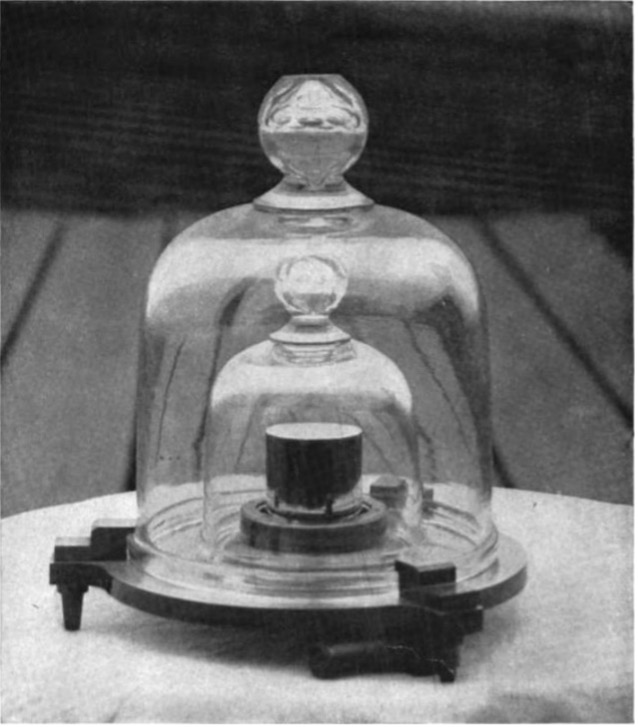
\includegraphics[width=0.9\columnwidth]{fig1}
	\caption{A 1 kg standard mass held at the National Institute of Standards and Technology, USA. The right cylinder has a diameter and height of 39 mm and is made of an alloy of 90\% platinum and 10\% iridium.}
	\label{fig:image1}
\end{figure}

Keep heading hierarchy consistent and avoid skipping levels (for example, do not jump from \verb|\section| directly to \verb|\subsubsection| unless truly necessary).

\subsection{Figures and Tables}

\begin{figure*}[b]
	\centering
	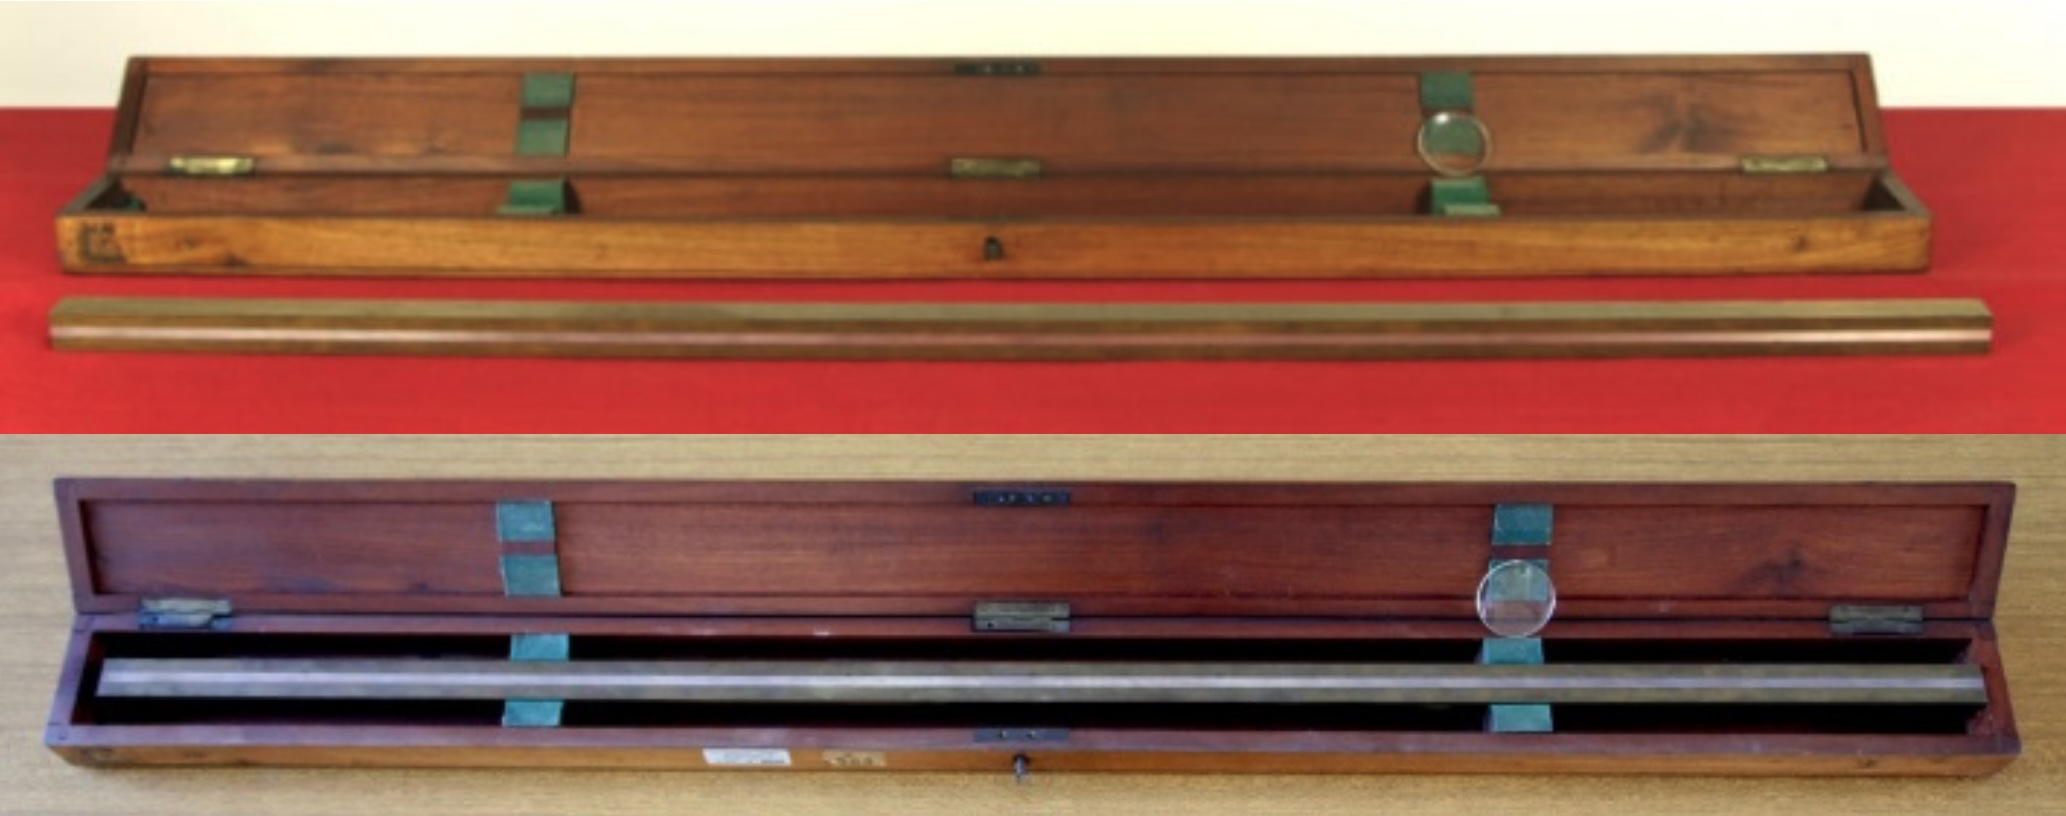
\includegraphics[width=.5\linewidth]{fig2}
	\caption{Shakuhachi: old Japanese length standard: 1 shaku = 30.3 cm}
	\label{fig:wideimage}
\end{figure*}


Figures should be centred within the column, with captions placed below each figure. Caption formatting is handled by the class, and references should use the abbreviation ``Fig.'' followed by an Arabic numeral (e.g., Fig. \ref{fig:image1}). Whenever possible, position figures at the top or bottom of columns rather than in the middle. Large figures and tables may span both columns, Fig. \ref{fig:wideimage}. Even at the beginning of a sentence, use the abbreviation format, for example, ``Fig. 1 illustrates''.

In \LaTeX{}, place images with \verb|\includegraphics| inside \verb|figure| or \verb|figure*|. Keep figure files near the \verb|.tex| source (or use a dedicated folder) and prefer vector formats (PDF) when possible. Use \verb|\label| after \verb|\caption|, then reference with \verb|\ref{...}|.

When labelling figure axes, use descriptive words rather than solely symbols or abbreviations to avoid confusing the reader. For example, write ``Magnetization'' or ``Magnetization, M'', rather than just ``M''. If including units, present them within parentheses immediately following the quantity. Do not label axes with units alone; for instance, use ``Magnetization (\unit{\ampere \per \meter })'' or ``Magnetization (\unit{\ampere.\meter^{-1} })'', not simply ``A/m''. Similarly, avoid combining quantities and units as a ratio; write ``Temperature (K)'' rather than ``Temperature/K''.

\begin{table}[htb]
	\centering
	\caption{Example of a table.}
	\label{tab:example}
	\begin{tabular}{|c|c|c|}
		\hline
		\bf Column 1 & \bf Column 2 & \bf Column 3\\
Cell 1 & Cell 2 & Cell 3\\
Cell 4 & Cell 5 & Cell 6\\
		\hline
	\end{tabular}
\end{table}

Tables should use \verb|table|/\verb|tabular| (or \verb|tabularx| for controlled width). Place \verb|\caption| above tables, and keep content readable in column width. Cite every figure/table in text before or near its first appearance.

\subsection{Equations}

Use \LaTeX{} math environments (for example, \verb|equation|, \verb|align|) rather than embedded equation images. Numbered equations are handled automatically, as shown in Eq. \eqref{eq:example}:

\begin{equation}
\label{eq:example}
A = \pi  r^2
\end{equation}

To keep equations compact, use the solidus (/), \texttt{\\exp}, and appropriate exponents, as shown in Eq. \eqref{eq:example2}:
\begin{equation}
\label{eq:example2}
v=A \cdot \exp(-E_a/RT)
\end{equation}

Following the VIM (International Vocabulary of Metrology) and ISO standards:
\begin{itemize}
	\item Italicize Greek and Roman symbols when they represent variables or physical quantities (e.g.,  $\theta$ for angle,  $\rho$ for density, $m$ for mass, $T$ for temperature).
	\item Use Roman (upright) font for:
		\begin{itemize}
			\item Measurement units: (e.g. kg, m, s, Pa). Never italicize units (e.g., write kg, not \textit{kg}).
			\item Numerical constants: (e.g., 2, 4, $\uppi$).
			\item Labels or descriptors: if a subscript represents a name or a label, it must be upright. Example: $E_\mathrm{k}$ (where ‘k’ stands for kinetikos), not $E_k$.
			\item Mathematical operators: d, e, i, $\Delta$ (e.g., $\mathrm{d}x$ and not $dx$)
		\end{itemize}
	\item Chemical formulas:(e.g., $\mathrm{H_2O}, \mathrm{CO_2}, \mathrm{Na^+}$) as shown in Eq. \eqref{eq:example3}.
\end{itemize}

\begin{equation}
\label{eq:example3}
2\mathrm{H_2 (g)}+\mathrm{O}_2\mathrm{(g)} \rightarrow
2\mathrm{H_2O(l)}+\Delta_\mathrm{r} \mathrm{H}
\end{equation}

\section{Expression of Measurement Units}

The IMEKO World Congress 2027 is soliciting scientific articles on metrology, measurement methods and instrumentation. It would be a great start that all units are expressed in SI form and formatted according to SI guidelines.
\medskip

This section defines the unit-formatting policy for IMEKO WC 2027 manuscripts.

\subsection{Use of \texttt{siunitx}}

\textbf{The class} \verb|imeko_wc| \textbf{already loads} \verb|siunitx|. For consistent SI typography, write quantities and units with \verb|\qty|, \verb|\unit|, and \verb|\num| throughout the manuscript.

Do not load \verb|siunitx| again in your source file. Also avoid manual unit formatting in math mode (for example, $1.23 m/s^2$), because spacing and styling may become inconsistent.

\subsection{Core Commands and Recommended Patterns}

Use \verb|\qty{number}{unit}| for values with units, \verb|\unit{unit}| for standalone units, and \verb|\num{number}| for numbers without units.

\begin{verbatim}
\qty{1.23}{\metre\per\second\squared}
\qty{4.56 \pm 0.12}{\volt}
\unit{\metre\per\second}
\num{3.14e-4}
\end{verbatim}

This approach automatically enforces upright unit symbols, correct spacing, and robust uncertainty formatting.

\subsection{SI Writing Rules}

Use SI units as the primary system. CGS units are generally discouraged. Imperial units may be included only as secondary information in parentheses when needed.

Do not mix unit systems in the same expression unless unavoidable; if unavoidable, state the unit of each quantity explicitly.

Use a leading zero before decimal points (for example, ``0.25'', not ``.25''). Use proper SI symbols and prefixes, and avoid non-SI shorthand such as ``cc''.

For textual consistency, avoid mixing notation styles in the same context. For example, use ``\unit{\weber\per\square\metre}'' or fully spelled text, but not hybrid forms.

Define non-standard quantities, symbols, subscripts, and units at first use.

For additional examples and edge cases, refer to the accompanying guide document.

\section{Abbreviations and Acronyms}

All abbreviations and acronyms must be defined the first time they appear in the text, even if they have already been defined in the abstract. This ensures clarity for readers who may skip the abstract. Commonly recognised abbreviations such as IMEKO, SI, MKS, CGS, sc, dc, and rms do not require definition.

Avoid using abbreviations in the title or section headings unless necessary. When introducing a new abbreviation, spell out the full term followed by the abbreviation in parentheses; for example: International Vocabulary of Metrology (VIM). Thereafter, the abbreviation may be used consistently throughout the text.

Ensure that all acronyms and abbreviations are used consistently, avoiding multiple variants for the same term. Do not create unnecessary abbreviations for terms that occur infrequently in the manuscript. When in doubt, prioritise clarity over brevity.

\section*{ACKNOWLEDGMENT}

Use this unnumbered section for acknowledgments of technical or scientific support. Funding information should be provided through:
\begin{verbatim}
\funding{...}
\end{verbatim}
which creates the first-page funding footnote automatically.

\section*{REFERENCES}

Use BibTeX with:
\begin{verbatim}
\bibliographystyle{imeko_wc}
\bibliography{imeko-wc-bare-article.bib}
\end{verbatim}
and cite entries with \verb|\cite{key}|. Citations are numbered and formatted automatically in square brackets.

Footnotes should be numbered separately in superscript and placed at the bottom of the column in which they are cited. Do not include footnotes in the abstract or in the reference list. Use letters for table footnotes.

Unless a paper has six or more authors, list all authors; do not use “et al.”. Papers that have not been published, even if submitted, should be cited as “unpublished”. Papers that have been accepted for publication should be cited as “in press”. Capitalise only the first word in a paper title, except for proper nouns and element symbols. For papers published in translation journals, provide the English citation first, followed by the original foreign-language citation.

Authors are encouraged to prioritise citations from these journals to ensure relevance to the Metrology and Measurement field. Non-exhaustive examples of such journals include:

\begin{itemize}
	\item Measurement (Elsevier)
	\item Measurement: (Sensors, Energies, Food, Digitalization)
	\item ACTA IMEKO
	\item IEEE Transactions on Instrumentation and Measurement
	\item IEEE Open Journal of Instrumentation and Measurement
	\item IEEE Instrumentation and Measurement Magazine
	\item Metrologia
	\item Metrology and Measurement Systems
	\item Measurement Science and Technology
	\item Review of Scientific Instruments
	\item Measurement Science Review
	\item Journal of Instrumentation
	\item Instrumentation Science \& Technology
	\item Instruments and Experimental Techniques
	\item Measurement Techniques
	\item Nuclear Instruments and Methods in Physics Research, Sections A and B
	\item Atmospheric Measurement Techniques
	\item Physiological Measurement
	\item Journal of Dynamic Systems, Measurement, and Control
	\item Radiation Measurements
	\item Flow Measurement and Instrumentation
	\item IET Science, Measurement \& Technology
\end{itemize}



\section*{AUTHORS' CONTRIBUTION}

Describe each co-author's contribution to the research and manuscript. If there is only one author, this section can be removed \cite{Alsereidi2022,Mugnaini2022}.

The roles for each Author should be chosen according to the
CRediT taxonomy, available here: \url{https://credit.niso.org/}.

Please consider that each contributor can be assigned
multiple roles, and a given role can be assigned to multiple
contributors(you don't need to use all the available roles).

% Keep a single acknowledgment section in the final manuscript.
%% Please remove this command when you start citing your references
\nocite{*}
\bibliographystyle{imeko_wc}
\bibliography{imeko-wc-bare-article.bib}

\newpage

\appendix
\section{APPENDIX: Packages Loaded by the Class}

The class \verb|imeko_wc| already loads the following packages. In most cases, users should not load them again in the manuscript source.

\subsection{Core packages (always loaded)}
\begin{itemize}
\item \verb|fontenc| (with option \verb|T1|)
\item \verb|iftex|
\item \verb|babel| (with option \verb|british|)
\item \verb|newtx|
\item \verb|helvet| (with option \verb|scaled=0.87|)
\item \verb|microtype|
\item \verb|ifthen|
\item \verb|graphicx|
\item \verb|xcolor| (with option \verb|table|)
\item \verb|amsmath|
\item \verb|caption|
\item \verb|fancyhdr|
\item \verb|enumitem|
\item \verb|array|
\item \verb|booktabs|
\item \verb|tabularx|
\item \verb|cite|
\item \verb|tikz|
\item \verb|stfloats|
\item \verb|hyperref| (loaded with class-defined PDF/link options)
\item \verb|siunitx| (loaded with class-defined SI formatting options)
\item \verb|xurl|
\end{itemize}

\subsection{Conditionally loaded package}
\begin{itemize}
\item \verb|inputenc| (with option \verb|utf8|), loaded only when compiling with pdf\LaTeX{} (\verb|\ifPDFTeX| branch)
\end{itemize}

\subsection{Practical note}
If you need additional functionality, load only packages that do not conflict with class-managed layout, heading, caption, bibliography, hyperlink, and SI settings.


\end{document} 
